\documentclass[conference]{IEEEtran}
\IEEEoverridecommandlockouts
\usepackage{cite}
\usepackage{amsmath,amssymb}
\usepackage{graphicx}
\usepackage{booktabs}
\usepackage{multirow}
\usepackage{xcolor}
\usepackage{tikz}
\usetikzlibrary{positioning,arrows.meta,fit,backgrounds}
\usepackage[hidelinks]{hyperref}
\graphicspath{{figs/}}
\makeatletter\newcommand\tabinput[1]{\@@input #1 }\makeatother
\newcommand{\Rronecvcontacts}{1.47}
\newcommand{\Rronecvfault}{0.00}
\newcommand{\Rronecvfreeze}{13}
\newcommand{\Rronecvpushed}{0.42}
\newcommand{\Rronecvreached}{88}
\newcommand{\Rronecvsuccess}{48}
\newcommand{\Rronecvtime}{23.3}
\newcommand{\Rronecvunivcontacts}{3.00}
\newcommand{\Rronecvunivsuccess}{15}
\newcommand{\Rronecvvsrtwocvci}{[-0.93, -0.30]}
\newcommand{\Rronecvvsrtwocvd}{-0.60}
\newcommand{\Rronecvvsrtwocvp}{0.010}
\newcommand{\Rronenonecontacts}{2.28}
\newcommand{\Rronenonefault}{0.00}
\newcommand{\Rronenonefreeze}{19}
\newcommand{\Rronenonepushed}{0.66}
\newcommand{\Rronenonereached}{88}
\newcommand{\Rronenonesuccess}{25}
\newcommand{\Rronenonetime}{23.8}
\newcommand{\Rronenoneunivcontacts}{4.17}
\newcommand{\Rronenoneunivsuccess}{2}
\newcommand{\Rrtwocvcontacts}{0.87}
\newcommand{\Rrtwocvfault}{0.45}
\newcommand{\Rrtwocvfreeze}{1}
\newcommand{\Rrtwocvpushed}{0.24}
\newcommand{\Rrtwocvreached}{92}
\newcommand{\Rrtwocvsuccess}{50}
\newcommand{\Rrtwocvtime}{25.2}
\newcommand{\Rrtwocvunivcontacts}{1.43}
\newcommand{\Rrtwocvunivsuccess}{20}
\newcommand{\Rrtwocvvsrtwolstmci}{[-0.12, +0.28]}
\newcommand{\Rrtwocvvsrtwolstmd}{+0.06}
\newcommand{\Rrtwocvvsrtwolstmp}{0.815}
\newcommand{\Rrtwocvvsrthreecvci}{[-0.38, -0.03]}
\newcommand{\Rrtwocvvsrthreecvd}{-0.20}
\newcommand{\Rrtwocvvsrthreecvp}{0.017}
\newcommand{\Rrtwokalmancontacts}{0.84}
\newcommand{\Rrtwokalmanfault}{0.40}
\newcommand{\Rrtwokalmanfreeze}{1}
\newcommand{\Rrtwokalmanpushed}{0.23}
\newcommand{\Rrtwokalmanreached}{90}
\newcommand{\Rrtwokalmansuccess}{53}
\newcommand{\Rrtwokalmantime}{24.5}
\newcommand{\Rrtwokalmanunivcontacts}{1.35}
\newcommand{\Rrtwokalmanunivsuccess}{22}
\newcommand{\Rrtwolstmcontacts}{0.93}
\newcommand{\Rrtwolstmfault}{0.41}
\newcommand{\Rrtwolstmfreeze}{1}
\newcommand{\Rrtwolstmpushed}{0.27}
\newcommand{\Rrtwolstmreached}{90}
\newcommand{\Rrtwolstmsuccess}{52}
\newcommand{\Rrtwolstmtime}{24.7}
\newcommand{\Rrtwolstmunivcontacts}{1.43}
\newcommand{\Rrtwolstmunivsuccess}{22}
\newcommand{\Rrtwononecontacts}{1.23}
\newcommand{\Rrtwononefault}{0.18}
\newcommand{\Rrtwononefreeze}{1}
\newcommand{\Rrtwononepushed}{0.47}
\newcommand{\Rrtwononereached}{91}
\newcommand{\Rrtwononesuccess}{41}
\newcommand{\Rrtwononetime}{24.0}
\newcommand{\Rrtwononeunivcontacts}{1.82}
\newcommand{\Rrtwononeunivsuccess}{20}
\newcommand{\Rrtwononevsrtwocvci}{[-0.61, -0.11]}
\newcommand{\Rrtwononevsrtwocvd}{-0.36}
\newcommand{\Rrtwononevsrtwocvp}{0.011}
\newcommand{\Rrtwosgcnncontacts}{0.78}
\newcommand{\Rrtwosgcnnfault}{0.34}
\newcommand{\Rrtwosgcnnfreeze}{1}
\newcommand{\Rrtwosgcnnpushed}{0.24}
\newcommand{\Rrtwosgcnnreached}{90}
\newcommand{\Rrtwosgcnnsuccess}{51}
\newcommand{\Rrtwosgcnntime}{23.8}
\newcommand{\Rrtwosgcnnunivcontacts}{1.27}
\newcommand{\Rrtwosgcnnunivsuccess}{20}
\newcommand{\Rrtwotcncontacts}{0.77}
\newcommand{\Rrtwotcnfault}{0.39}
\newcommand{\Rrtwotcnfreeze}{1}
\newcommand{\Rrtwotcnpushed}{0.27}
\newcommand{\Rrtwotcnreached}{88}
\newcommand{\Rrtwotcnsuccess}{53}
\newcommand{\Rrtwotcntime}{23.2}
\newcommand{\Rrtwotcnunivcontacts}{1.20}
\newcommand{\Rrtwotcnunivsuccess}{20}
\newcommand{\Rrthreecvcontacts}{0.67}
\newcommand{\Rrthreecvcpfivezerocontacts}{0.78}
\newcommand{\Rrthreecvcpfivezerofault}{0.46}
\newcommand{\Rrthreecvcpfivezerofreeze}{3}
\newcommand{\Rrthreecvcpfivezeropushed}{0.18}
\newcommand{\Rrthreecvcpfivezeroreached}{83}
\newcommand{\Rrthreecvcpfivezerosuccess}{47}
\newcommand{\Rrthreecvcpfivezerotime}{25.4}
\newcommand{\Rrthreecvcpfivezerounivcontacts}{1.25}
\newcommand{\Rrthreecvcpfivezerounivsuccess}{20}
\newcommand{\Rrthreecvcpsevenzerocontacts}{0.88}
\newcommand{\Rrthreecvcpsevenzerofault}{0.49}
\newcommand{\Rrthreecvcpsevenzerofreeze}{3}
\newcommand{\Rrthreecvcpsevenzeropushed}{0.15}
\newcommand{\Rrthreecvcpsevenzeroreached}{73}
\newcommand{\Rrthreecvcpsevenzerosuccess}{41}
\newcommand{\Rrthreecvcpsevenzerotime}{27.4}
\newcommand{\Rrthreecvcpsevenzerounivcontacts}{1.45}
\newcommand{\Rrthreecvcpsevenzerounivsuccess}{8}
\newcommand{\Rrthreecvcpninezerocontacts}{0.78}
\newcommand{\Rrthreecvcpninezerofault}{0.48}
\newcommand{\Rrthreecvcpninezerofreeze}{6}
\newcommand{\Rrthreecvcpninezeropushed}{0.10}
\newcommand{\Rrthreecvcpninezeroreached}{55}
\newcommand{\Rrthreecvcpninezerosuccess}{35}
\newcommand{\Rrthreecvcpninezerotime}{31.6}
\newcommand{\Rrthreecvcpninezerounivcontacts}{1.27}
\newcommand{\Rrthreecvcpninezerounivsuccess}{0}
\newcommand{\Rrthreecvfault}{0.47}
\newcommand{\Rrthreecvfreeze}{2}
\newcommand{\Rrthreecvpushed}{0.23}
\newcommand{\Rrthreecvreached}{93}
\newcommand{\Rrthreecvreplaycontacts}{0.92}
\newcommand{\Rrthreecvreplayfault}{0.45}
\newcommand{\Rrthreecvreplayfreeze}{2}
\newcommand{\Rrthreecvreplaypushed}{0.00}
\newcommand{\Rrthreecvreplayreached}{93}
\newcommand{\Rrthreecvreplaysuccess}{48}
\newcommand{\Rrthreecvreplaytime}{23.0}
\newcommand{\Rrthreecvreplayunivcontacts}{1.25}
\newcommand{\Rrthreecvreplayunivsuccess}{28}
\newcommand{\Rrthreecvreplayvsrthreecvci}{[-0.37, -0.13]}
\newcommand{\Rrthreecvreplayvsrthreecvd}{-0.25}
\newcommand{\Rrthreecvreplayvsrthreecvp}{0.002}
\newcommand{\Rrthreecvsuccess}{52}
\newcommand{\Rrthreecvtime}{23.6}
\newcommand{\Rrthreecvunivcontacts}{0.80}
\newcommand{\Rrthreecvunivsuccess}{30}
\newcommand{\Rrthreecvvsrthreecvcpfivezeroci}{[-0.05, +0.29]}
\newcommand{\Rrthreecvvsrthreecvcpfivezerod}{+0.12}
\newcommand{\Rrthreecvvsrthreecvcpfivezerop}{0.309}
\newcommand{\Rrthreecvvsrthreecvcpninezeroci}{[-0.12, +0.35]}
\newcommand{\Rrthreecvvsrthreecvcpninezerod}{+0.12}
\newcommand{\Rrthreecvvsrthreecvcpninezerop}{0.397}
\newcommand{\Rrthreecvvsrthreekalmanci}{[-0.05, +0.23]}
\newcommand{\Rrthreecvvsrthreekalmand}{+0.08}
\newcommand{\Rrthreecvvsrthreekalmanp}{0.964}
\newcommand{\Rrthreecvvsrthreelstmci}{[-0.03, +0.23]}
\newcommand{\Rrthreecvvsrthreelstmd}{+0.10}
\newcommand{\Rrthreecvvsrthreelstmp}{0.360}
\newcommand{\Rrthreecvvsrthreemlpci}{[-0.03, +0.24]}
\newcommand{\Rrthreecvvsrthreemlpd}{+0.11}
\newcommand{\Rrthreecvvsrthreemlpp}{0.480}
\newcommand{\Rrthreecvvsrthreesfci}{[-0.03, +0.23]}
\newcommand{\Rrthreecvvsrthreesfd}{+0.10}
\newcommand{\Rrthreecvvsrthreesfp}{0.227}
\newcommand{\Rrthreecvvsrthreesgcnnci}{[-0.04, +0.26]}
\newcommand{\Rrthreecvvsrthreesgcnnd}{+0.10}
\newcommand{\Rrthreecvvsrthreesgcnnp}{0.580}
\newcommand{\Rrthreecvvsrthreetcnci}{[-0.03, +0.24]}
\newcommand{\Rrthreecvvsrthreetcnd}{+0.10}
\newcommand{\Rrthreecvvsrthreetcnp}{0.420}
\newcommand{\Rrthreekalmancontacts}{0.75}
\newcommand{\Rrthreekalmanfault}{0.56}
\newcommand{\Rrthreekalmanfreeze}{2}
\newcommand{\Rrthreekalmanpushed}{0.23}
\newcommand{\Rrthreekalmanreached}{91}
\newcommand{\Rrthreekalmansuccess}{57}
\newcommand{\Rrthreekalmantime}{23.2}
\newcommand{\Rrthreekalmanunivcontacts}{1.12}
\newcommand{\Rrthreekalmanunivsuccess}{35}
\newcommand{\Rrthreelstmcontacts}{0.77}
\newcommand{\Rrthreelstmcpfivezerocontacts}{0.86}
\newcommand{\Rrthreelstmcpfivezerofault}{0.48}
\newcommand{\Rrthreelstmcpfivezerofreeze}{2}
\newcommand{\Rrthreelstmcpfivezeropushed}{0.18}
\newcommand{\Rrthreelstmcpfivezeroreached}{80}
\newcommand{\Rrthreelstmcpfivezerosuccess}{48}
\newcommand{\Rrthreelstmcpfivezerotime}{24.9}
\newcommand{\Rrthreelstmcpfivezerounivcontacts}{1.38}
\newcommand{\Rrthreelstmcpfivezerounivsuccess}{20}
\newcommand{\Rrthreelstmcpsevenzerocontacts}{0.77}
\newcommand{\Rrthreelstmcpsevenzerofault}{0.43}
\newcommand{\Rrthreelstmcpsevenzerofreeze}{4}
\newcommand{\Rrthreelstmcpsevenzeropushed}{0.13}
\newcommand{\Rrthreelstmcpsevenzeroreached}{72}
\newcommand{\Rrthreelstmcpsevenzerosuccess}{45}
\newcommand{\Rrthreelstmcpsevenzerotime}{27.1}
\newcommand{\Rrthreelstmcpsevenzerounivcontacts}{1.27}
\newcommand{\Rrthreelstmcpsevenzerounivsuccess}{12}
\newcommand{\Rrthreelstmcpninezerocontacts}{0.88}
\newcommand{\Rrthreelstmcpninezerofault}{0.45}
\newcommand{\Rrthreelstmcpninezerofreeze}{6}
\newcommand{\Rrthreelstmcpninezeropushed}{0.11}
\newcommand{\Rrthreelstmcpninezeroreached}{55}
\newcommand{\Rrthreelstmcpninezerosuccess}{32}
\newcommand{\Rrthreelstmcpninezerotime}{31.7}
\newcommand{\Rrthreelstmcpninezerounivcontacts}{1.35}
\newcommand{\Rrthreelstmcpninezerounivsuccess}{0}
\newcommand{\Rrthreelstmfault}{0.47}
\newcommand{\Rrthreelstmfreeze}{1}
\newcommand{\Rrthreelstmpushed}{0.25}
\newcommand{\Rrthreelstmreached}{97}
\newcommand{\Rrthreelstmsuccess}{52}
\newcommand{\Rrthreelstmtime}{24.3}
\newcommand{\Rrthreelstmunivcontacts}{1.10}
\newcommand{\Rrthreelstmunivsuccess}{28}
\newcommand{\Rrthreemlpcontacts}{0.78}
\newcommand{\Rrthreemlpfault}{0.45}
\newcommand{\Rrthreemlpfreeze}{2}
\newcommand{\Rrthreemlppushed}{0.28}
\newcommand{\Rrthreemlpreached}{93}
\newcommand{\Rrthreemlpsuccess}{52}
\newcommand{\Rrthreemlptime}{23.4}
\newcommand{\Rrthreemlpunivcontacts}{1.07}
\newcommand{\Rrthreemlpunivsuccess}{25}
\newcommand{\Rrthreenonecontacts}{1.47}
\newcommand{\Rrthreenonefault}{0.37}
\newcommand{\Rrthreenonefreeze}{2}
\newcommand{\Rrthreenonepushed}{0.47}
\newcommand{\Rrthreenonereached}{86}
\newcommand{\Rrthreenonesuccess}{36}
\newcommand{\Rrthreenonetime}{26.0}
\newcommand{\Rrthreenoneunivcontacts}{2.27}
\newcommand{\Rrthreenoneunivsuccess}{12}
\newcommand{\Rrthreenonevsrthreecvci}{[-1.10, -0.51]}
\newcommand{\Rrthreenonevsrthreecvd}{-0.80}
\newcommand{\Rrthreenonevsrthreecvp}{$<$0.001}
\newcommand{\Rrthreesfcontacts}{0.77}
\newcommand{\Rrthreesffault}{0.51}
\newcommand{\Rrthreesffreeze}{1}
\newcommand{\Rrthreesfpushed}{0.24}
\newcommand{\Rrthreesfreached}{92}
\newcommand{\Rrthreesfsuccess}{52}
\newcommand{\Rrthreesftime}{23.0}
\newcommand{\Rrthreesfunivcontacts}{1.02}
\newcommand{\Rrthreesfunivsuccess}{30}
\newcommand{\Rrthreesgcnncontacts}{0.77}
\newcommand{\Rrthreesgcnnfault}{0.51}
\newcommand{\Rrthreesgcnnfreeze}{1}
\newcommand{\Rrthreesgcnnpushed}{0.26}
\newcommand{\Rrthreesgcnnreached}{91}
\newcommand{\Rrthreesgcnnsuccess}{56}
\newcommand{\Rrthreesgcnntime}{22.8}
\newcommand{\Rrthreesgcnnunivcontacts}{1.20}
\newcommand{\Rrthreesgcnnunivsuccess}{32}
\newcommand{\Rrthreetcncontacts}{0.77}
\newcommand{\Rrthreetcnfault}{0.47}
\newcommand{\Rrthreetcnfreeze}{2}
\newcommand{\Rrthreetcnpushed}{0.27}
\newcommand{\Rrthreetcnreached}{92}
\newcommand{\Rrthreetcnsuccess}{52}
\newcommand{\Rrthreetcntime}{23.8}
\newcommand{\Rrthreetcnunivcontacts}{1.15}
\newcommand{\Rrthreetcnunivsuccess}{28}
\newcommand{\Rrhoaccsafe}{-0.71}
\newcommand{\Rrhoaccsafep}{0.07}


\begin{document}

\title{Does Better Pedestrian Prediction Make a Safer Robot?\\
A Predictor, Uncertainty and Planner Benchmark on Real Crowds}

\author{\IEEEauthorblockN{Filmon Nezif Abamecha}
\IEEEauthorblockA{Higher Colleges of Technology\\
United Arab Emirates}}

\maketitle

\begin{abstract}
Robots that cross pedestrian areas rely on trajectory prediction, yet
predictors are usually judged by displacement error rather than by how
safely a robot drives with them. We build a complete navigation stack in
MATLAB with a classical and a learned option at each layer: seven
predictors (constant velocity, Kalman, Social Force, MLP, LSTM, temporal
CNN and a social-grid CNN), split and adaptive conformal uncertainty, 2-D
and space-time A*, and pure pursuit, dynamic-window and sampling-based MPC
controllers. We evaluate 23 configurations on the same 120 episodes from
the ETH/UCY scenes, using a leak-free split and a reactive Social Force
crowd that follows the recorded routes. Prediction halves the contacts of
a space-time planner (1.47 to 0.67 per episode), and space-time A* with
MPC has 54\% fewer contacts than A* with pure pursuit. However, the learned
predictors are up to 10\% more accurate but no safer than constant
velocity: no paired difference is significant. Conformal margins lose
their 90\% coverage under the shift to an unseen scene and, used as hard
constraints, cut goal-reaching from 93\% to 55\% without reducing
contacts. The planner, not the predictor, is the lever for safety.

\end{abstract}

\begin{IEEEkeywords}
crowd navigation, trajectory prediction, conformal prediction, model predictive control, space-time A*, social force
\end{IEEEkeywords}

\section{Introduction}
A mobile robot that crosses a pedestrian area has to answer three
questions every fraction of a second: where will each person be, how sure
is that guess, and which motion keeps the robot clear of everyone while
still making progress? Each question has a large literature. Trajectory
predictors have moved from hand-made models such as Social Force
\cite{helbing1995} to recurrent, generative and graph networks
\cite{alahi2016,gupta2018,salzmann2020,rudenko2020}. Conformal prediction
gives distribution-free error bounds that can be wrapped around any
predictor \cite{vovk2005,lindemann2023,dixit2023}. Planners range from
grid search and reactive controllers \cite{hart1968,fox1997} to model
predictive control in space and time \cite{mavrogiannis2023}.

These layers are usually studied one at a time. Prediction papers report
displacement errors on ETH/UCY \cite{pellegrini2009,lerner2007} and stop
there, even though a constant-velocity model is already hard to beat on
those scenes \cite{scholler2020}. Navigation papers report collisions but
often use one predictor. Poddar et al.\ \cite{poddar2023} showed that a
model predictive controller drove about as safely with constant-velocity
prediction as with a deep generative predictor. That raises the question
this paper studies:
\emph{when a whole navigation stack is held fixed, how much does a more
accurate predictor, a calibrated uncertainty margin, or a better planner
change how safely and smoothly a robot crosses a real crowd?}

We answer it with one controlled benchmark built end to end in MATLAB.
The contributions are:
\begin{itemize}
\item a complete, open stack with a classical and a learned option at each
layer: Kalman tracking, seven predictors (constant velocity, Kalman,
Social Force, MLP, LSTM, temporal CNN and a social-grid CNN), split and
adaptive conformal uncertainty, 2-D and space-time A*, and pure pursuit,
dynamic-window and sampling-based MPC controllers;
\item a leak-free ETH/UCY protocol and a reactive Social Force crowd that
follows the recorded routes but yields to the robot, so contacts can be
attributed to the robot or to the person;
\item a paired benchmark of 23 stack configurations on the same 120
episodes, with bootstrap confidence intervals, which shows that the planner
and controller dominate, that predictor accuracy is only weakly linked to
safety, and how conformal margins trade contacts against freezing.
\end{itemize}
The code, trained weights and every number in this paper can be
reproduced with the public repository.\footnote{\url{https://github.com/filmonnezif/crowd-nav-matlab}}

\section{Related Work}
\textbf{Prediction.} Social Force \cite{helbing1995} models people as
particles pushed by goals and neighbours. Social LSTM \cite{alahi2016},
Social GAN \cite{gupta2018} and Trajectron++ \cite{salzmann2020} learn the
interaction from data; Rudenko et al.\ \cite{rudenko2020} survey the field.
Sch\"oller et al.\ \cite{scholler2020} showed that constant velocity
matches many deep models on ETH/UCY, so we keep it as the reference.
Temporal convolutions \cite{bai2018} are a light alternative to recurrent
networks \cite{hochreiter1997}.

\textbf{Uncertainty.} Split conformal prediction \cite{vovk2005} turns
validation errors into a radius that holds with probability $1-\alpha$ if
test data is exchangeable with calibration data. Adaptive conformal
inference (ACI) \cite{gibbs2021} adjusts the level online under shift.
Lindemann et al.\ \cite{lindemann2023} and Dixit et al.\ \cite{dixit2023}
use such radii as constraints in MPC. Gaussian processes
\cite{rasmussen2006} and the Kalman covariance \cite{kalman1960} give
model-based alternatives.

\textbf{Planning in crowds.} A* \cite{hart1968} with pure pursuit
\cite{coulter1992} or the dynamic window approach (DWA) \cite{fox1997} is
the classical mobile-robot stack. Space-time search \cite{silver2005} lets
a planner wait for a gap. Trautman and Krause \cite{trautman2010} named
the \emph{freezing robot problem}: when every future looks possible, every
path looks blocked. Mavrogiannis et al.\ \cite{mavrogiannis2023} review
the open problems of social navigation, including evaluation with
non-reactive replayed crowds, which we address with a reactive crowd.

\section{System}
Fig.~\ref{fig:system} shows the stack. Every layer has the same
interface, so any predictor can be combined with any uncertainty method,
planner and controller.

\begin{figure}[t]
\centering
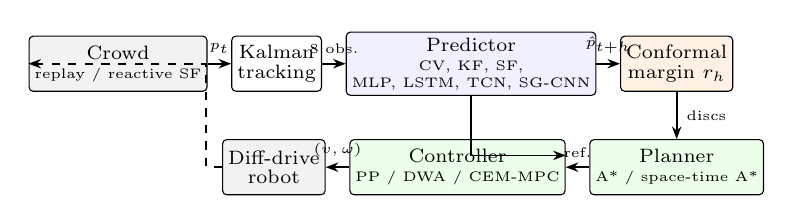
\begin{tikzpicture}[font=\scriptsize, node distance=3.5mm and 3mm,
  box/.style={draw, rounded corners=1.5pt, align=center, minimum height=7mm, inner sep=2pt, fill=white},
  arr/.style={-{Stealth[length=1.6mm]}, semithick}]
\node[box, fill=gray!10] (crowd) {Crowd\\[-1pt]{\tiny replay / reactive SF}};
\node[box, right=of crowd] (kf) {Kalman\\[-1pt]tracking};
\node[box, right=of kf, fill=blue!6] (pred) {Predictor\\[-1pt]{\tiny CV, KF, SF,}\\[-2pt]{\tiny MLP, LSTM, TCN, SG-CNN}};
\node[box, right=of pred, fill=orange!10] (cp) {Conformal\\[-1pt]margin $r_h$};
\node[box, below=6mm of cp, fill=green!8] (plan) {Planner\\[-1pt]{\tiny A* / space-time A*}};
\node[box, left=of plan, fill=green!8] (ctrl) {Controller\\[-1pt]{\tiny PP / DWA / CEM-MPC}};
\node[box, left=of ctrl, fill=gray!10] (robot) {Diff-drive\\[-1pt]robot};
\draw[arr] (crowd) -- node[above]{\tiny $p_t$} (kf);
\draw[arr] (kf) -- node[above]{\tiny 8 obs.} (pred);
\draw[arr] (pred) -- node[above]{\tiny $\hat p_{t+h}$} (cp);
\draw[arr] (cp) -- node[right]{\tiny discs} (plan);
\draw[arr] (pred.south) |- ([yshift=1.5mm]ctrl.east);
\draw[arr] (plan) -- node[above]{\tiny ref.} (ctrl);
\draw[arr] (ctrl) -- node[above]{\tiny $(v,\omega)$} (robot);
\draw[arr, dashed] (robot.west) -- ++(-2mm,0) |- (crowd.west);
\end{tikzpicture}
\caption{Navigation stack. The robot's motion feeds back into the reactive
crowd (dashed). Prediction runs every 0.4\,s for 12 steps (4.8\,s).}
\label{fig:system}
\end{figure}

\subsection{Data and protocol}
We use the six standard ETH/UCY scenes \cite{pellegrini2009,lerner2007}
(ETH, Hotel, Zara1, Zara2, Univ students001/003), sampled at 2.5\,Hz.
A prediction window is 8 observed and 12 future positions (3.2\,s and
4.8\,s). The usual split, which takes the last 20\% of windows of each
scene as validation, leaks: 978 validation windows share frames with
training windows. We instead choose one split time per scene and drop
windows that straddle it, which gives 28{,}022 training, 4{,}634
validation and 364 ETH test windows with no overlap. ETH is held out from
training and calibration; learned models are tuned on validation only.

\subsection{Predictors}
\emph{Constant velocity} (CV) extrapolates the last observed step.
\emph{Kalman} runs a constant-velocity filter \cite{kalman1960} over the
track and rolls it forward. \emph{Social Force} (SF) \cite{helbing1995}
simulates everyone jointly with repulsion from people ahead; its strength
and range are tuned on validation. The four networks work in each
person's \emph{heading frame} (origin at the person, $x$ along the walking
direction) and output a \emph{residual} over CV for all 12 steps, which
keeps a zero-output network equal to the baseline. The MLP (38k
parameters) sees the 7 flattened displacements, the LSTM
\cite{hochreiter1997} (64 units, 29k) sees them as a sequence, the
temporal CNN \cite{bai2018} (63k) applies dilated 1-D convolutions, and the
social-grid CNN (58k) adds a 2-D CNN over a $16\times16$ grid of
neighbours' positions and velocities (0.5\,m cells). They are trained
with mirrored augmentation (56k samples) and early stopping. For
simulation, the trained weights are exported and run with plain matrix
code that matches the toolbox to within $10^{-4}$\,m.

\subsection{Conformal uncertainty}
For a predictor $f$ and horizon $h$, let $e_{i,h}=\|\hat p_{i,h}-p_{i,h}\|$
on the $n$ validation windows. Split conformal prediction takes
$q_h$ as the $\lceil (n+1)(1-\alpha)\rceil$-th smallest score, so a disc
of radius $q_h$ contains the truth with probability at least $1-\alpha$
under exchangeability \cite{vovk2005}. Because walking speed changes the
error scale, we use the normalised score $e_{i,h}/(0.5+s_i)$ with $s_i$ the
person's speed, so that $r_{i,h}=(0.5+s_i)\,q_h$. ACI \cite{gibbs2021}
updates $\alpha$ online on the test stream instead. The planner sees each
predicted person as a disc of radius $r_{\text{ped}}+r_{\text{robot}}+r_{i,h}$.

\subsection{Planners and controllers}
\textbf{2-D A*} \cite{hart1968} plans every 0.4\,s on a 0.25\,m grid. A
predicted position $\tau$ seconds ahead is a hard obstacle where the robot
could meet the person ($|d-v_{\max}\tau|<1$\,m) and a soft cost elsewhere.
\textbf{Space-time A*} (ST-A*) \cite{silver2005} copies a 0.3\,m grid for
12 time layers of 0.4\,s. From each cell the robot can wait or move to a
neighbour, and a cell is blocked at a layer if a predicted disc covers it
then. Because every edge moves forward in time the graph is acyclic, so
the optimal plan is found exactly by vectorised backward dynamic
programming in about 20\,ms. Its output is a time-stamped reference, so a
\emph{wait} in the plan makes the reference stand still.

\textbf{Pure pursuit} (PP) \cite{coulter1992} follows the path with a
governor that slows and stops near people. \textbf{DWA} \cite{fox1997}
scores 77 $(v,\omega)$ commands (including slow reversing) reachable within
0.4\,s, rolled out for 2\,s against the predicted people, on progress,
clearance, speed and smoothness. \textbf{CEM-MPC} optimises 8 commands of
0.4\,s with the cross-entropy method \cite{rubinstein2004} (120 samples,
3 iterations, 10\% elite, warm start). Its cost is tracking the plan's
time-stamped reference, a clearance penalty against the predicted discs at
the matching times, and smoothness. The robot is a unicycle of radius
0.3\,m with $v_{\max}=1$\,m/s and $\omega_{\max}=2$\,rad/s, simulated at
10\,Hz.

We evaluate three robots: \textbf{R1} = A* + PP, \textbf{R2} = A* + DWA, and
\textbf{R3} = ST-A* + CEM-MPC.

\subsection{Reactive crowd and metrics}
A replayed crowd never yields, so a robot that stops is walked into. In
our \emph{reactive} crowd each recorded person is simulated with Social
Force: they steer towards where the recording has them 1.2\,s later, are
repelled by the robot and by each other (anisotropically, with a
pass-on-the-right component), and are limited to 2\,m/s. Without a robot
the simulated crowd stays 0.21\,m from the recording on average.
Predictors observe the simulated crowd, never the ground truth future.

An episode starts the robot 1\,m inside one end of the scene's long axis
with the goal 1\,m inside the other end, so it has to cross the main
pedestrian flow within 60\,s. Each scene gives 10 start times in
both directions, for 120 episodes. We report: \emph{success} (goal reached
with no contact), \emph{reached} (goal within the limit), \emph{contacts}
per episode (body overlap events), \emph{at-fault} contacts (the robot was
closing in at more than 0.1\,m/s), time to goal, the share of time
stopped, and \emph{people pushed}: how far, in metres, the robot displaced
people from where the same simulated crowd walks without it. All
configurations run the same 120 episodes, so differences are
\emph{paired}; we give 95\% bootstrap intervals and Wilcoxon signed-rank
$p$-values.

\section{Experiments and Results}
\begin{table}[t]
\centering
\caption{Prediction error (m) for 12 steps (4.8\,s). ETH is never seen in training or calibration.}
\label{tab:pred}
\setlength{\tabcolsep}{4pt}
\begin{tabular}{lcccc}
\toprule
& \multicolumn{2}{c}{Validation} & \multicolumn{2}{c}{ETH test}\\
\cmidrule(lr){2-3}\cmidrule(lr){4-5}
Predictor & ADE & FDE & ADE & FDE\\
\midrule
Constant velocity & 0.440 & 0.972 & 1.075 & 2.282\\
Kalman CV & 0.443 & 0.977 & 1.071 & 2.277\\
Social Force & 0.461 & 0.993 & 1.056 & 2.238\\
MLP & 0.431 & 0.938 & 1.030 & 2.091\\
LSTM & 0.440 & 0.958 & \textbf{1.003} & \textbf{2.045}\\
Temporal CNN & 0.430 & 0.936 & 1.021 & 2.058\\
Social-grid CNN & \textbf{0.429} & \textbf{0.934} & 1.044 & 2.155\\
\bottomrule
\end{tabular}
\end{table}

\begin{table}[t]
\centering
\caption{90\% uncertainty discs on ETH: empirical coverage and mean radius (m) at 1.6/3.2/4.8\,s.}
\label{tab:cov}
\setlength{\tabcolsep}{3.5pt}
\begin{tabular}{llcc}
\toprule
Pred. & Method & Coverage & Radius 1.6 / 3.2 / 4.8 s\\
\midrule
CV & split conformal & 57\% & 0.48 / 1.25 / 2.18\\
CV & speed-normalised conformal & 64\% & 0.65 / 1.74 / 3.03\\
CV & ACI & 90\% & 2.39 / 6.04 / 11.9\\
Kalman & filter covariance & 98\% & 1.84 / 4.85 / 8.69\\
LSTM & speed-normalised conformal & 65\% & 0.63 / 1.67 / 2.88\\
LSTM & ACI & 90\% & 1.67 / 3.74 / 6.86\\
GP & predictive $\sigma$ & 61\% & 0.49 / 1.28 / 2.23\\
\bottomrule
\end{tabular}
\end{table}

\begin{table*}[t]
\centering
\caption{Navigation in the reactive crowd, 120 paired episodes per row. Contacts per episode with 95\% bootstrap interval.
Univ = mean contacts in the two dense university scenes. Time = mean time to goal when reached. Pushed = people displaced by the robot (m).}
\label{tab:nav}
\setlength{\tabcolsep}{5pt}
\begin{tabular}{lcccccccc}
\toprule
Predictor & ETH ADE (m) & Success (\%) & Reached (\%) & Contacts / ep & At-fault / ep & Univ contacts & Time (s) & Pushed (m)\\
\midrule
\tabinput{generated/tab_nav.tex}
\bottomrule
\end{tabular}
\end{table*}

\begin{table}[t]
\centering
\caption{Conformal margins in R3 (ST-A* + MPC). Level = coverage target of the speed-normalised disc.}
\label{tab:margin}
\setlength{\tabcolsep}{3pt}
\begin{tabular}{llcccccc}
\toprule
Pred. & Level & Succ. & Reach. & Cont. & Univ succ. & Stop & Pushed\\
& & (\%) & (\%) & /ep & (\%) & (\%) & (m)\\
\midrule
\tabinput{generated/tab_margin.tex}
\bottomrule
\end{tabular}
\end{table}


\subsection{Prediction and calibration}
Table~\ref{tab:pred} confirms the known picture \cite{scholler2020}: the
three classical predictors are within 5\% of each other, and every network
beats them, by about 10\% in FDE on the unseen ETH scene. The social-grid
CNN, which sees the neighbours, is best on validation, while the LSTM
transfers best to ETH.

Table~\ref{tab:cov} shows that the conformal guarantee does not survive
the move to ETH. People there walk about twice as fast as in the
validation scenes (median 1.01 vs 0.51\,m/s), so 90\% discs calibrated on
validation cover only 57--65\% of ETH. Normalising by speed recovers 7
points. ACI restores 90\% coverage, but ETH errors are heavy-tailed and
the discs grow to several metres. Here the better predictor pays off: with
ACI the LSTM needs discs about 30\% smaller than CV for the same coverage.
Model-based uncertainty is either over-confident (GP, 61\%) or very
conservative (Kalman, 98\% with discs 3--4$\times$ larger).

\subsection{Navigation}
Table~\ref{tab:nav} and Fig.~\ref{fig:acc} give the main result. With 120
episodes a success rate has a standard error of about 4.5 points, so we
compare contacts, which are paired and more sensitive.

\emph{Using any prediction helps, and helps more the better the planner
can use it.} Constant-velocity prediction lowers contacts from 2.28 to
1.47 per episode with R1, from 1.23 to 0.87 with R2 ($-0.36$, 95\% CI
$[-0.61,-0.11]$, $p=0.011$) and from 1.47 to 0.67 with R3 ($-0.80$,
$[-1.10,-0.51]$, $p<0.001$). Without prediction, ST-A* is worse than
2-D A*: a space-time plan built on people standing still is confidently
wrong. With prediction it is the best planner.

\emph{The planner and controller matter more than the predictor.} With CV
prediction, replacing pure pursuit by DWA removes 0.60 contacts per episode
($[-0.93,-0.30]$, $p=0.010$), and replacing 2-D A* + DWA by ST-A* + MPC
removes another 0.20 ($[-0.38,-0.03]$, $p=0.017$). In the dense
university scenes contacts fall from 3.00 to 1.43 to 0.80 per episode and
success rises from 15\% to 20\% to 30\%. Pure pursuit is never at fault,
but it stops in people's way 13\% of the time and pushes them most
(0.42\,m); DWA and MPC almost never stop and disturb people about half as
much, at the cost of 0.4--0.5 at-fault contacts per episode.

\emph{Prediction accuracy does not translate into safety.} In R3, every
other predictor has slightly \emph{more} contacts than CV (0.75--0.78 vs
0.67), and no paired difference is significant ($+0.08$ to $+0.11$,
$p\ge0.23$). In R2 the predictors range from 0.77 to 0.93 contacts with
no link to accuracy: the LSTM, best on ETH, is last. Across the seven R3
predictors the rank correlation between ETH FDE and contacts is
$\rho=-0.71$ ($p=0.07$), i.e.\ if anything the less accurate predictors
are safer. Goal-reaching and time are also flat (LSTM reaches the goal
most often, 97\%, and the social-grid CNN is fastest, 22.8\,s). This
extends the finding of Poddar et al.\ \cite{poddar2023} from one deep
predictor to six predictors and three planners.

\emph{Replayed crowds overstate the risk.} The same R3 with CV has 0.92
contacts per episode when people are replayed and 0.67 when they react
($-0.25$, $[-0.37,-0.13]$, $p=0.002$), while at-fault contacts stay at
0.45--0.47: the extra contacts in replay are people walking into the
robot.

\begin{figure}[t]
\centering
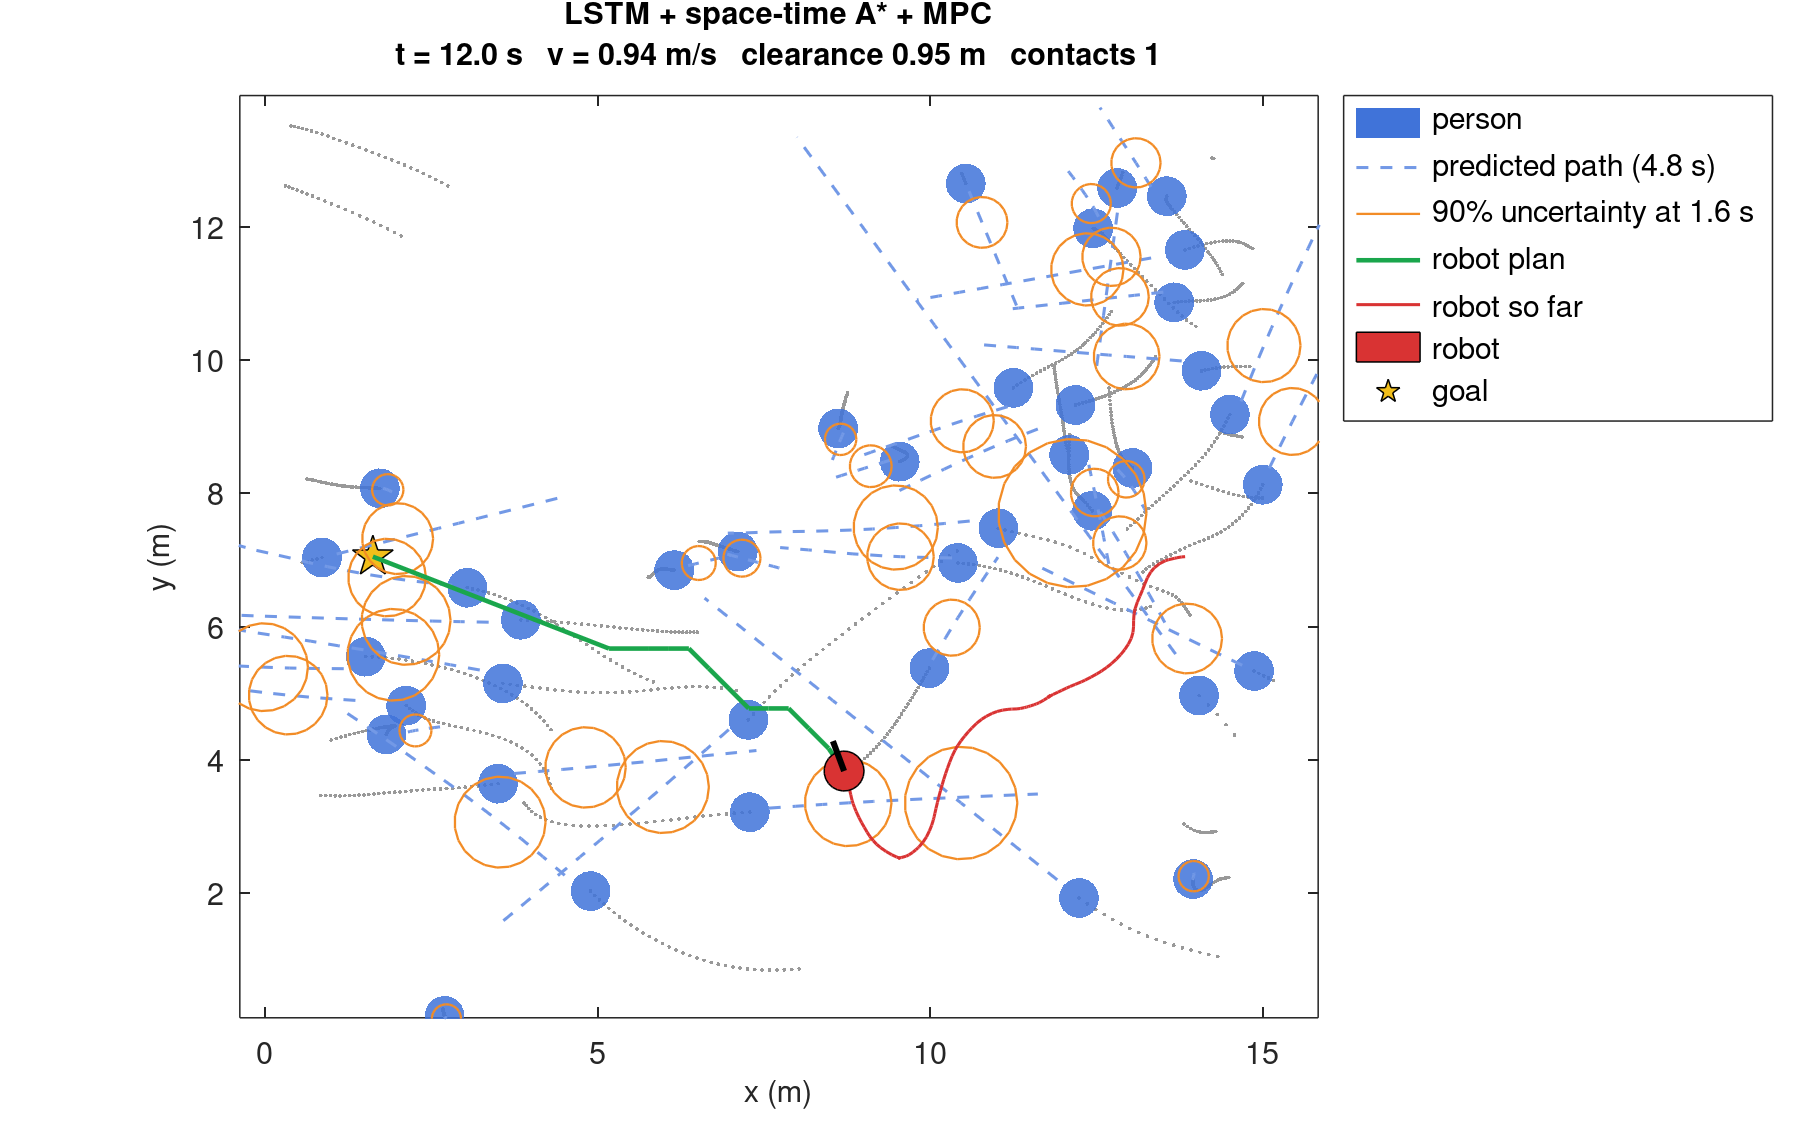
\includegraphics[width=\columnwidth]{fig_scene.png}
\caption{Students003 at $t=12$\,s with R3 and the LSTM predictor. Dashed:
4.8\,s LSTM predictions; orange: 90\% conformal discs at 1.6\,s (shown,
not used by this planner); green: space-time plan; red: path driven so
far; grey: recorded routes.}
\label{fig:scene}
\end{figure}

\begin{figure}[t]
\centering
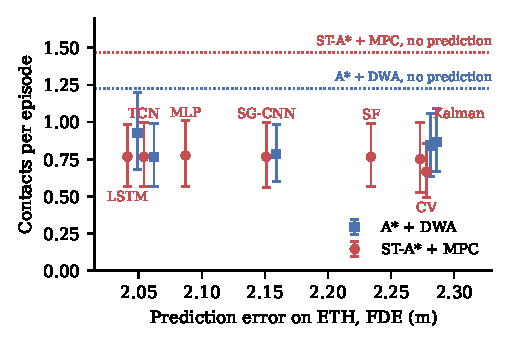
\includegraphics[width=\columnwidth]{fig_acc_safety.pdf}
\caption{Prediction error on ETH against contacts per episode (95\%
bootstrap intervals). Dotted lines: the same robot without prediction.}
\label{fig:acc}
\end{figure}

\begin{figure}[t]
\centering
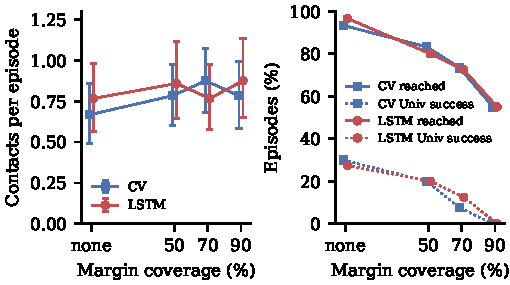
\includegraphics[width=\columnwidth]{fig_margin.pdf}
\caption{Conformal margins in R3. Left: contacts per episode (95\%
bootstrap intervals). Right: goal reached (solid) and success in the
university scenes (dotted).}
\label{fig:margin}
\end{figure}

\subsection{Uncertainty margins}
Table~\ref{tab:margin} and Fig.~\ref{fig:margin} add speed-normalised
conformal discs to every predicted person in R3. The margins make the robot
more cautious, as intended: people are displaced less (0.23 to
0.10\,m) and it stops more (1.5\% to 5.9\%). But they do not reduce
contacts. For CV, contacts go from 0.67 to 0.78, 0.88 and 0.78 at 50, 70
and 90\% coverage ($p=0.31$ and $0.40$ for 50\% and 90\%), and the LSTM
behaves the same way. Meanwhile the goal is reached in 93\%, 83\%, 73\%
and 55\% of episodes, success in the university scenes falls from 30\%
to 0\%, and travel time rises from 23.6 to 31.6\,s. This is the freezing
robot problem \cite{trautman2010}: with 90\% discs a fast walker's disc
is several metres wide at 3\,s, the space-time grid is blocked, and the
robot waits while people still reach it. With a replayed crowd and DWA
the same margins did cut contacts by about 20\% (1.06 to 0.86) in our
earlier runs; once people yield, the margins mostly cost progress.

\section{Discussion and Limitations}
\textbf{Why does accuracy not help?} Three effects combine. First, the
planner uses predictions only up to 3.2\,s ahead, and the gap between
predictors grows with the horizon; the 10\% FDE gain is at 4.8\,s.
Second, contacts in a reactive crowd are dominated by close-range
interaction, which the inflated hard obstacles and the controller's
clearance cost already handle. Third, the networks were trained on
recorded people who never met a robot. In our crowd people swerve
around the robot, and a model that smooths 8 observations (Kalman,
networks) reacts to a swerve later than CV, which uses only the last
step. Predictors trained or adapted in closed loop with the robot are the
natural next step.

\textbf{Where uncertainty helps.} Calibrated discs are only useful if the
planner can still move inside them. Under the ETH shift, guaranteed
coverage costs metres of room (Table~\ref{tab:cov}). A better predictor
shrinks the ACI discs by 30\%, which is the one place where accuracy paid
off in our study, and risk-weighted costs instead of hard discs
\cite{lindemann2023,dixit2023} are a promising way to use them.

\textbf{Limitations.} The crowd is a Social Force model driven by the
recordings, not real people; its reaction to a robot is a modelling
choice. All results are in simulation on six scenes, with one robot
model and 120 episodes per configuration, which resolves differences of
about 0.2 contacts per episode but not smaller ones. The networks are
small and deterministic; multi-modal generative predictors
\cite{gupta2018,salzmann2020} may behave differently.

\section{Conclusion}
We built a complete crowd-navigation stack in MATLAB with classical and
learned options at every layer, a leak-free ETH/UCY protocol and a
reactive crowd, and compared 23 configurations on the same 120 episodes.
Prediction itself matters: it halves contacts for a space-time planner.
But \emph{which} predictor matters little: six predictors that differ by
up to 10\% in displacement error give statistically identical navigation,
and the simplest is at least as safe. The choice of planner and controller
changes safety far more, with space-time A* and sampling MPC reducing
contacts by 54\% against A* with pure pursuit. Conformal margins are
calibrated only in distribution and, used as hard constraints, freeze the
robot in dense scenes. Navigation benchmarks should therefore report
closed-loop safety in reactive crowds, not displacement error alone.
Code, weights and results are public.



\bibliographystyle{IEEEtran}
\bibliography{refs}

\end{document}
